\documentclass[../main.tex]{subfiles}

\begin{document}

This project has been developed in the context of Xmipp and Scipion framework. The image processing algorithms have been implemented inside Xmipp, whilst the refinement logic has been implemented in the Xmipp's Scipion plugin.

The image processing part implemented in Xmipp has been named as \textit{swiftalign}, the union of the words \textit{swift} and \textit{align}. This name precisely describes the purpose of these programs: Fast image alignment. The \textit{swiftalign} framework implements two programs: \texttt{swiftalign\_train} and \texttt{swiftalign\_query}. 

These two programs, along other Xmipp programs, will be invoked from the Scipion protocol named as \textit{swiftres}. This protocol is used to implement the refinement logic. This means that it will be responsible of orchestrating calls to the image processing algorithms and provide an easy to use \gls{gui} for the end user.

\subsection{swiftalign\_train}

\subsection{swiftalign\_query}

\subsection{swiftres}

\begin{figure}[hbpt]
    \centering
    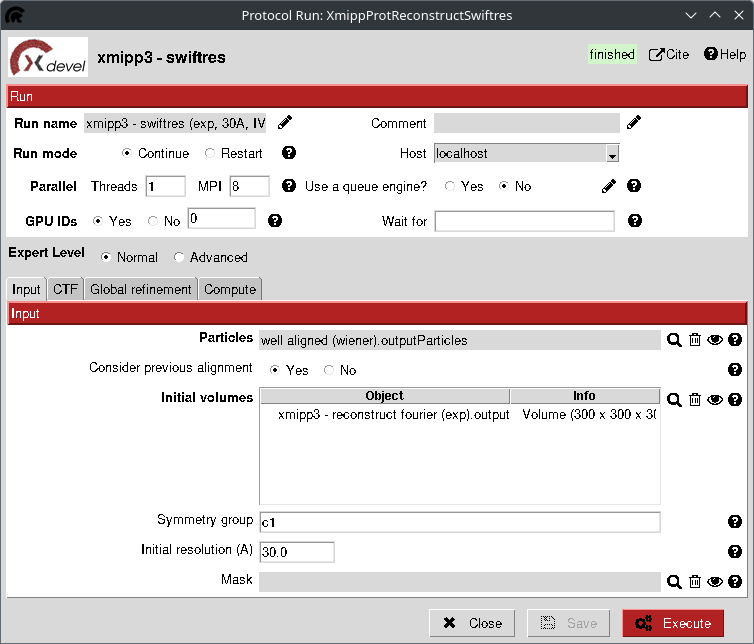
\includegraphics[width=.8\textwidth]{implementation/form}
    \caption{Screenshot of the user interface for running \textit{swiftres} protocol in Scipion}
    \label{fig:my_label}
\end{figure}

\end{document}
